\documentclass[10pt]{article}
\usepackage{geometry, graphicx, listings, subfigure, setspace} 
\usepackage[usenames,dvipsnames]{xcolor}

\graphicspath{{./figure/}}
\DeclareGraphicsExtensions{.pdf, .jepg, .png, .jpg}
\lstset{
    language=C++,                                % 设置语言为C++
    basicstyle=\ttfamily\small,                  % 设置基本样式为等宽字体,小号字体
    keywordstyle=\color{blue},                   % 设置关键字颜色为蓝色
    stringstyle=\color{orange},                  % 设置字符串颜色为橙色
    commentstyle=\color{green!60!black},         % 设置注释颜色为绿色
    identifierstyle=\color{black},               % 设置标识符颜色为黑色
    numbers=left,                                % 行号显示在左侧
    numberstyle=\tiny\color{gray},               % 设置行号样式为小号灰色
    stepnumber=1,                                % 每行显示行号
    numbersep=5pt,                               % 行号与代码的距离
    backgroundcolor=\color{white},               % 设置背景颜色为白色
    showspaces=false,                            % 不显示空格
    showstringspaces=false,                      % 不显示字符串中的空格
    showtabs=false,                              % 不显示制表符
    frame=single,                                % 设置代码框为单线边框
    tabsize=4,                                   % 设置制表符大小为4个空格
    captionpos=b,                                % 设置标题位置为底部
    breaklines=true,                             % 自动换行
    breakatwhitespace=true,                      % 在空格处自动换行
    extendedchars=false,                         % 解决代码跨页时,章节标题,页眉等汉字不显示的问题
    morecomment=[l]{//},                         % 设置行注释符为//
    morecomment=[s]{/*}{*/},                     % 设置块注释符为/*和*/
    morekeywords={alignas, alignof, and, and_eq, asm, auto, bitand, bitor, bool, break, case, catch, char, char8_t, char16_t, char32_t, class, compl, concept, const, consteval, constexpr, const_cast, continue, co_await, co_return, co_yield, decltype, default, delete, do, double, dynamic_cast, else, enum, explicit, export, extern, false, float, for, friend, goto, if, inline, int, long, mutable, namespace, new, noexcept, not, not_eq, nullptr, operator, or, or_eq, private, protected, public, register, reinterpret_cast, requires, return, short, signed, sizeof, static, static_assert, static_cast, struct, switch, template, this, thread_local, throw, true, try, typedef, typeid, typename, union, unsigned, using, virtual, void, volatile, wchar_t, while, xor, xor_eq, {, }, (, ), <, >, <=, >=, ==, !=}, % 设置额外的关键字
}


\geometry{a4paper,left=2cm,right=2cm,top=2cm,bottom=2cm}
\title{COMP5822M High Performance Graphics Coursework 1 Report}
\author{Simiao Wang 201702881}
\date{\today}

\begin{document}

\maketitle

\noindent For the convenience of demonstration, change the `\#define VERSION 0` to other number in the `\#define` section of `current\_Version.hpp`, then compile and run.

\begin{lstlisting}
    #define DEFAULT 0
    #define MIPMAP_VISUALIZE_LINEAR 1
    #define MIPMAP_VISUALIZE_NEAREST 2
    #define FRAGMENT_DEPTH 3
    #define PARTIAL_DERIVATIVES_FRAGMENT_DEPTH 4
    #define ANISOTROPIC_FILTERING 5
    #define OVERDRAW_VISUALIZE 6
    #define OVERSHADING_VISUALIZE 7
    #define MESHDENSITY_VISUALIZE 8
    
    #define CURRENT_VERSION 0
\end{lstlisting}

\noindent The presetting to numbers here is because string comparison cannot be performed later in the \#if statement.

\section{Vulkan infrastructure}

\noindent Vulkan device name: NVIDIA GeForce RTX 3060 Laptop GPU

\noindent Vulkan Loader's versions: 1.3.277 (variant 0)

\noindent Device's Vulkan versions: 1.3.277

\noindent Extensions:VK\_KHR\_surface, VK\_KHR\_win32\_surface, VK\_EXT\_debug\_utils, VK\_KHR\_swapchain

\noindent Swap chain images\_Color format: VK\_FORMAT\_R8G8B8A8\_SRGB

\noindent Swap chain images\_Number of images: 3

\section{3D Scene and Navigation}

\subsection{The way to handle different meshes and materials}

\noindent If the mesh has textures, load their corresponding texture images and create texture image views.

\noindent If the mesh does not have textures, use the default sprite texture.

\noindent Create descriptor sets and allocate one for textured mesh. In the descriptor sets, bind information such as texture images and texture samplers to the corresponding descriptors.

\begin{lstlisting}
if(mesh.textured)
{
	std::vector<float> tempPos;
	std::vector<float> tempTex;
	for (std::size_t i = 0; i < mesh.vertexCount; i++)
	{
		tempPos.push_back(Model.dataTextured.positions[mesh.vertexStartIndex + i].x);
		tempPos.push_back(Model.dataTextured.positions[mesh.vertexStartIndex + i].y);
		tempPos.push_back(Model.dataTextured.positions[mesh.vertexStartIndex + i].z);
		tempTex.push_back(Model.dataTextured.texcoords[mesh.vertexStartIndex + i].x);
		tempTex.push_back(Model.dataTextured.texcoords[mesh.vertexStartIndex + i].y);
	}
	{
		lut::CommandPool loadCmdPool = lut::create_command_pool(window, VK_COMMAND_POOL_CREATE_TRANSIENT_BIT);
		modelTex.push_back(lut::load_image_texture2d(Model.materials[mesh.materialIndex].diffuseTexturePath.c_str(), window, loadCmdPool.handle, allocator));
		modelView.push_back(lut::create_image_view_texture2d(window, modelTex.back().image, VK_FORMAT_R8G8B8A8_SRGB));
	}
	tempDescriptors = lut::alloc_desc_set(window, dpool.handle, objectLayout.handle);
	{
		VkWriteDescriptorSet desc[1]{};
		VkDescriptorImageInfo textureInfo{};
		textureInfo.imageLayout = VK_IMAGE_LAYOUT_SHADER_READ_ONLY_OPTIMAL;
		textureInfo.imageView = modelView.back().handle;
		textureInfo.sampler = defaultSampler.handle;
		desc[0].sType = VK_STRUCTURE_TYPE_WRITE_DESCRIPTOR_SET;
		desc[0].dstSet = tempDescriptors;
		desc[0].dstBinding = 0;
		desc[0].descriptorType = VK_DESCRIPTOR_TYPE_COMBINED_IMAGE_SAMPLER;
		desc[0].descriptorCount = 1;
		desc[0].pImageInfo = &textureInfo;
		constexpr auto numSets = sizeof(desc) / sizeof(desc[0]);
		vkUpdateDescriptorSets(window.device, numSets, desc, 0, nullptr);
	}
	TexturedMesh tempMesh = create_model_mesh(window, allocator, tempPos, tempTex);
	modelMesh.push_back(std::move(tempMesh));
	modelDescriptors.push_back(std::move(tempDescriptors));
}
else
{
	std::vector<float> aircraftTempPos;
	std::vector<glm::vec3> aircraftColor;
	for (std::size_t i = 0; i < mesh.vertexCount; i++)
	{
		aircraftTempPos.push_back(Model.dataUntextured.positions[mesh.vertexStartIndex + i].x);
		aircraftTempPos.push_back(Model.dataUntextured.positions[mesh.vertexStartIndex + i].y);
		aircraftTempPos.push_back(Model.dataUntextured.positions[mesh.vertexStartIndex + i].z);
		aircraftColor.push_back(Model.materials[mesh.materialIndex].diffuseColor);
		aircraftColor.push_back(Model.materials[mesh.materialIndex].diffuseColor);
		aircraftColor.push_back(Model.materials[mesh.materialIndex].diffuseColor);
	}
	ColorizedMesh tempMesh = create_color_mesh(window, allocator, aircraftTempPos, aircraftColor);
	colorizedMesh.push_back(std::move(tempMesh));
}
\end{lstlisting}

\subsection{Loading time and per-frame operations.}

\noindent Loading: Load models, texture images, allocate descriptor sets, and create model mesh objects, update descriptor sets.

\begin{lstlisting}
    SimpleModel Model = load_simple_wavefront_obj(cfg::kModelPath);
    // other code
    for(auto const& mesh:Model.meshes)
    {
        // other code
    }
\end{lstlisting}

\noindent per-frame: Command buffers are recorded for rendering the scene.
Commands are submitted for execution using vkQueueSubmit().
Finally, the rendered images are presented to the screen using vkQueuePresentKHR().

\subsection{Relevant screenshots}

\noindent The final effect of task 1.2 is as shown in the Figure 1.

\begin{figure}[htbp]
    \centering
    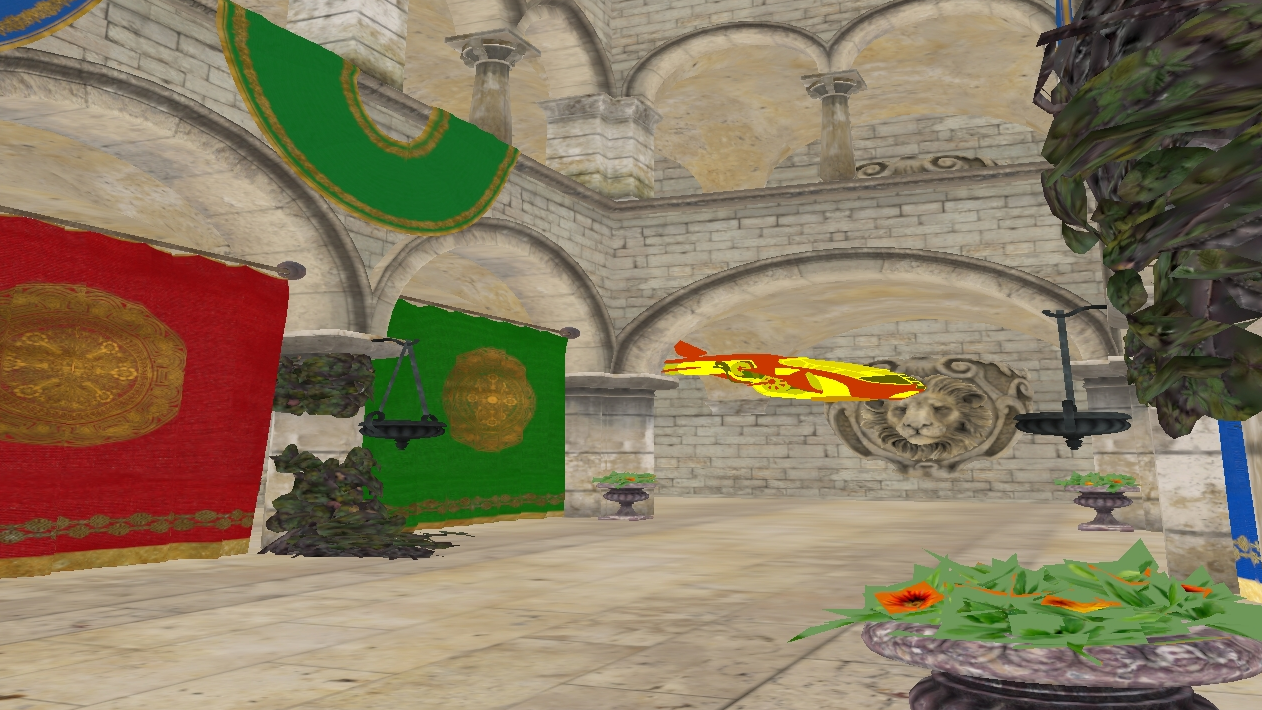
\includegraphics[width=9cm]{1.2.png}
    \caption{final effect of task 1.2}
\end{figure}

\section{Anisotropic filtering}

\noindent In `vulkan\_window.cpp`, add the following code in `create\_device()` function to enable anisotropic filtering.

\begin{lstlisting}
#if CURRENT_VERSION == ANISOTROPIC_FILTERING
    deviceFeatures.samplerAnisotropy = VK_TRUE;
#endif
\end{lstlisting}

\noindent In `vkutil.cpp`, add the following code in `create\_default\_sampler()` function. 

\begin{lstlisting}
#if CURRENT_VERSION == ANISOTROPIC_FILTERING
    samplerInfo.anisotropyEnable = VK_TRUE;
    samplerInfo.maxAnisotropy = 16.0f;
#endif
\end{lstlisting}

\noindent The final result is as shown in Figure 2. When enabling anisotropic filtering and setting maxAnisotropy to 16.0f, textures in the distance appear relatively clearer.

\begin{figure}[htbp]
	\centering
	\subfigure[On]{
        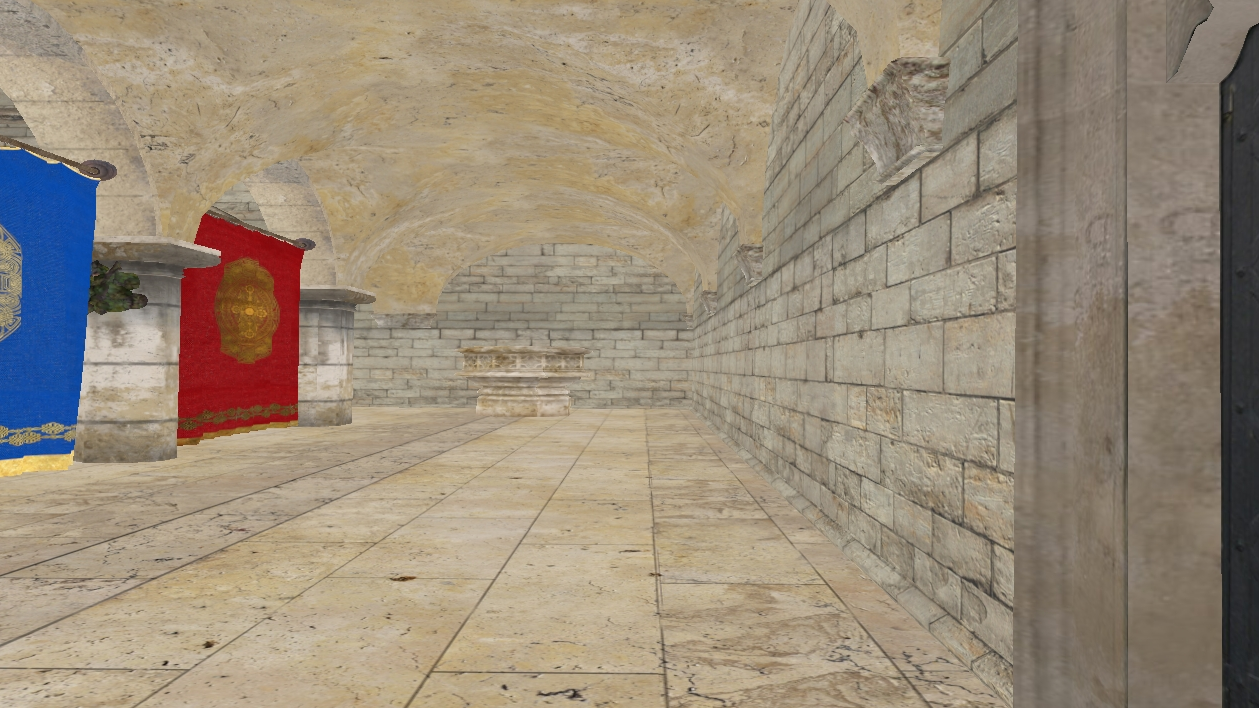
\includegraphics[width=0.45\textwidth]{1.3_ON.png}
    }
    \subfigure[Off]{
        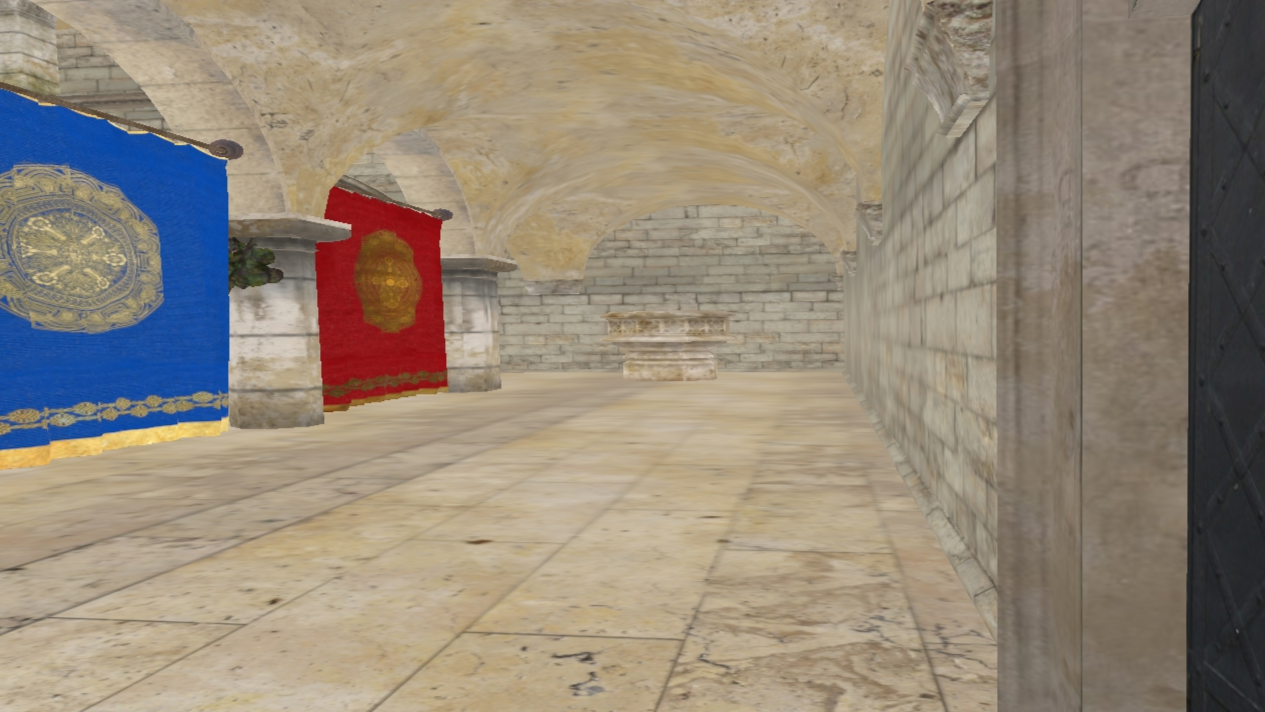
\includegraphics[width=0.45\textwidth]{1.3_OFF.png}
    }
    \caption{The difference between enabling or disabling anisotropic filtering}
\end{figure}

\section{Visualizing fragment properties}

\subsection{Utilization of texture mipmap levels}

\noindent In the `mipmapVisualize.frag`, I use `textureQueryLod(uTexColor, v2fTexCoord).x` to obtain the level of detail (LOD) value of the texture `uTexColor` at the texture coordinate `v2fTexCoord`. Then, I extract the integer and fractional parts of this LOD value, where the integer part represents the mipmap level, and the fractional part is used for interpolation. Finally, I output the interpolated result.

\begin{lstlisting}
    float lod = textureQueryLod(uTexColor, v2fTexCoord).x;
    float mipmapLevel = floor(lod); 
    float fraction = fract(lod); 
    vec4 colorA;
    vec4 colorB;

    if(mipmapLevel == 0.0) {
        colorA = vec4(1.0, 0.0, 0.0, 1.0);
        colorB = vec4(1.0, 1.0, 0.0, 1.0);
    } else if(mipmapLevel == 1.0) {
        colorA = vec4(1.0, 1.0, 0.0, 1.0);
        colorB = vec4(0.0, 1.0, 0.0, 1.0);
    } else if(mipmapLevel == 2.0) {
        colorA = vec4(0.0, 1.0, 0.0, 1.0);
        colorB = vec4(0.0, 1.0, 1.0, 1.0);
    } else if(mipmapLevel == 3.0) {
        colorA = vec4(0.0, 1.0, 1.0, 1.0);
        colorB = vec4(0.0, 0.0, 1.0, 1.0);
    } else if(mipmapLevel == 4.0) {
        colorA = vec4(0.0, 0.0, 1.0, 1.0);
        colorB = vec4(0.5, 0.0, 0.5, 1.0);
    } else if(mipmapLevel == 5.0) {
        colorA = vec4(0.5, 0.0, 0.5, 1.0); 
        colorB = vec4(1.0, 0.0, 1.0, 1.0); 
    } else if(mipmapLevel == 6.0) {
        colorA = vec4(1.0, 0.0, 1.0, 1.0); 
        colorB = vec4(1.0, 1.0, 1.0, 1.0); 
    } else {
        colorA = vec4(1.0, 1.0, 1.0, 1.0); 
        colorB = vec4(0.0, 0.0, 0.0, 1.0); 
    }

    oColor = mix(colorA, colorB, fraction);
\end{lstlisting}

\noindent When the default mipmap mode is LINEAR, the rendering results are as shown in Figure 3 for the default size, magnification, and reduction.
When enlarging the window, I noticed that lower Mipmap levels can be displayed, while when shrinking the window, I noticed that higher Mipmap levels can be displayed.

\noindent 推理得: 窗口的大小与显示的分辨率有关, 窗口越小, 实际分辨率就不需要太高, 所以就用高的mipmap level就足够了

\begin{figure}[htbp]
	\centering
	\subfigure[dufault size]{
        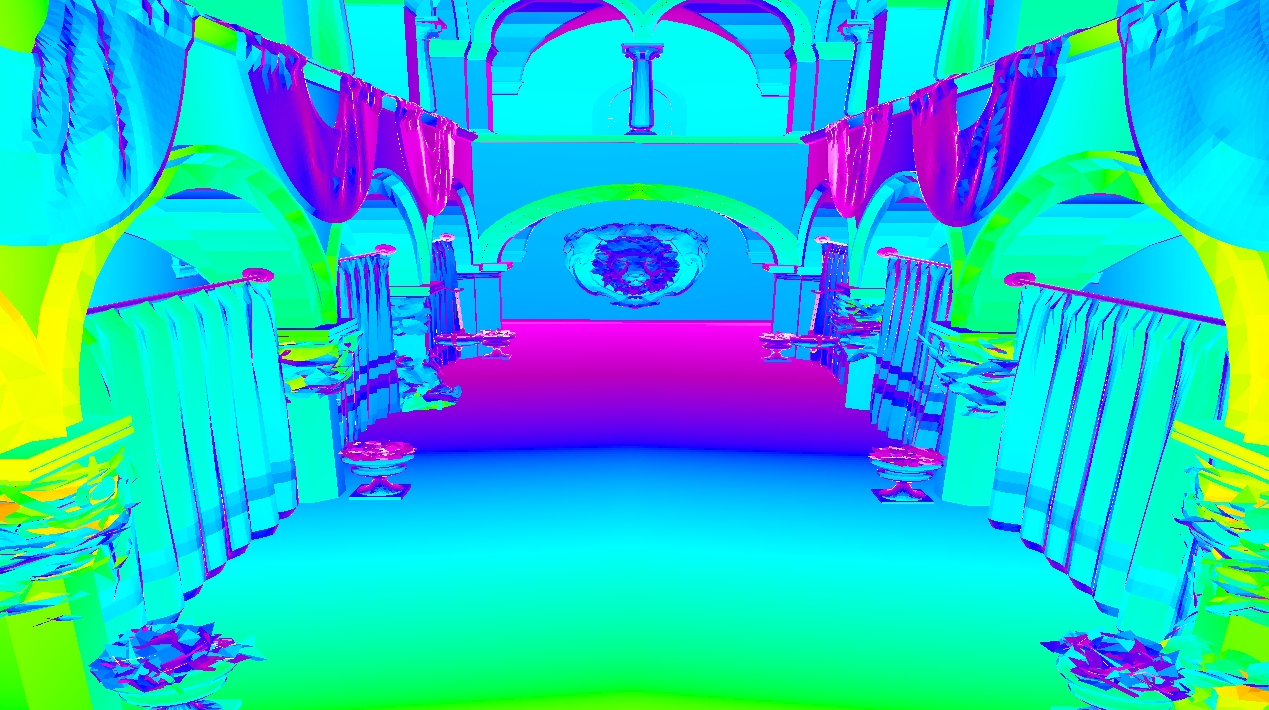
\includegraphics[width=0.3\textwidth]{1.4_mipmapLevels_default.png}
    }
    \subfigure[reduction]{
        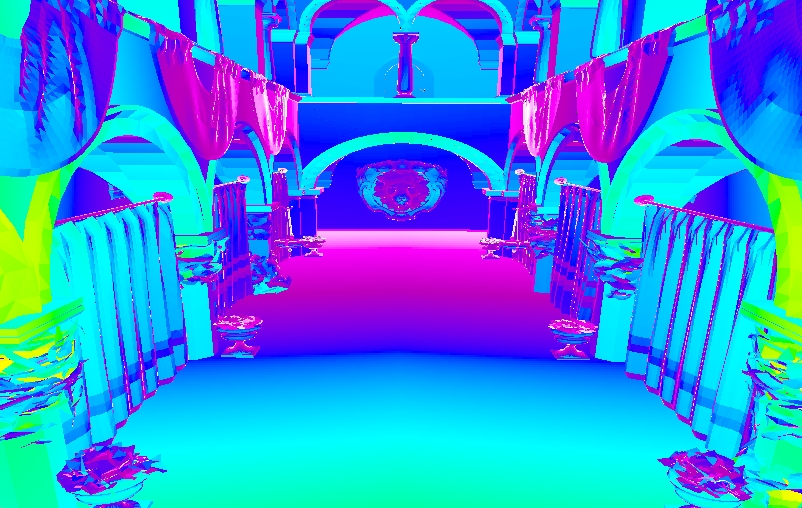
\includegraphics[width=0.2\textwidth]{1.4_mipmapLevels_mini.png}
    }
    \subfigure[magnification]{
        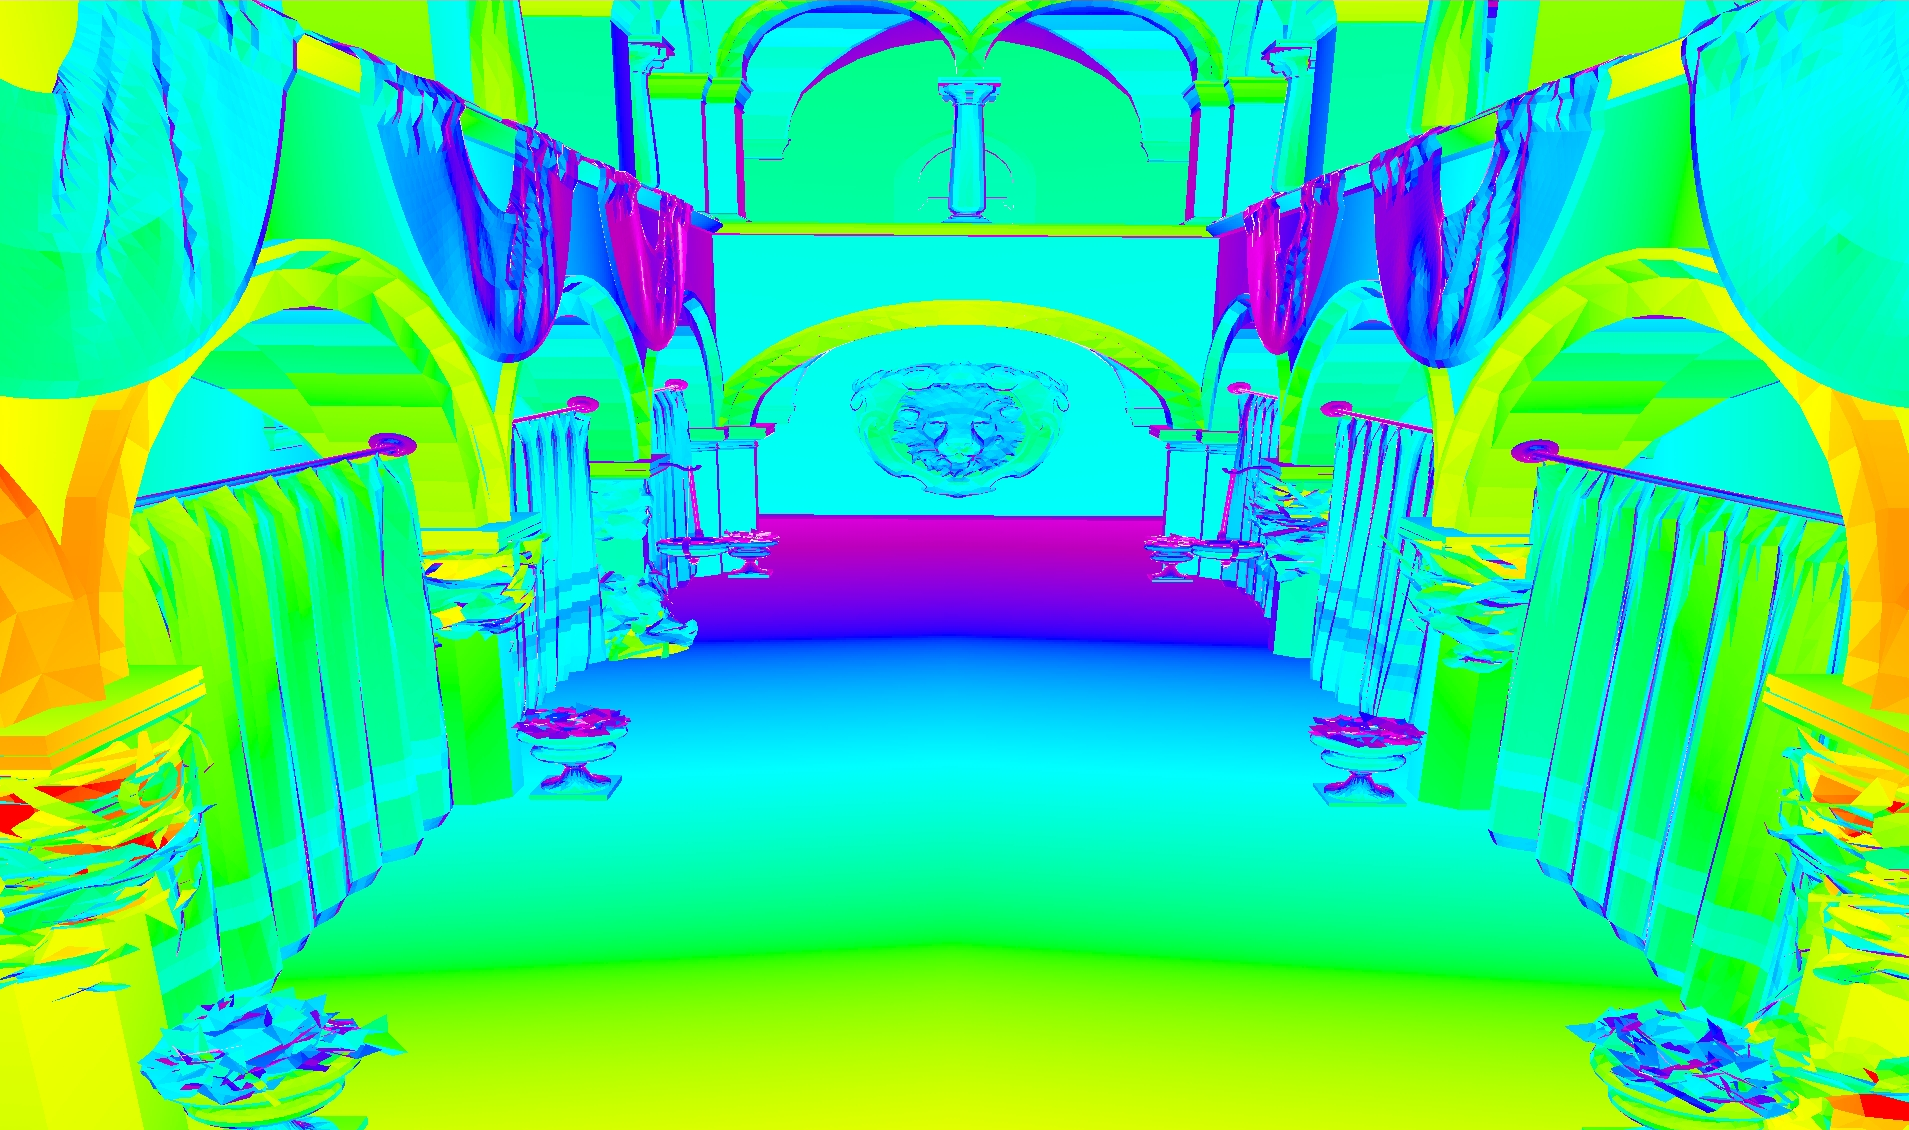
\includegraphics[width=0.4\textwidth]{1.4_mipmapLevels_blowup.png}
    }
    \caption{Mipmap mode is LINEAR}
\end{figure}

\noindent In the `create\_default\_sampler()` function in vkutil.cpp, different Mipmap modes can be obtained by modifying `samplerInfo.mipmapMode`.

\begin{lstlisting}
#if CURRENT_VERSION == MIPMAP_VISUALIZE_NEAREST
    samplerInfo.mipmapMode = VK_SAMPLER_MIPMAP_MODE_NEAREST;
#elif CURRENT_VERSION == MIPMAP_VISUALIZE_LINEAR
    samplerInfo.mipmapMode = VK_SAMPLER_MIPMAP_MODE_LINEAR;
#else
    samplerInfo.mipmapMode = VK_SAMPLER_MIPMAP_MODE_LINEAR;
#endif
\end{lstlisting}

\noindent The rendering results of the two Mipmap modes are shown in Figure 4.
 I noticed that the Mipmap transitions in LINEAR mode are smooth, while in NEAREST mode, the transitions are not smooth.

\begin{figure}[htbp]
	\centering
	\subfigure[LINEAR]{
        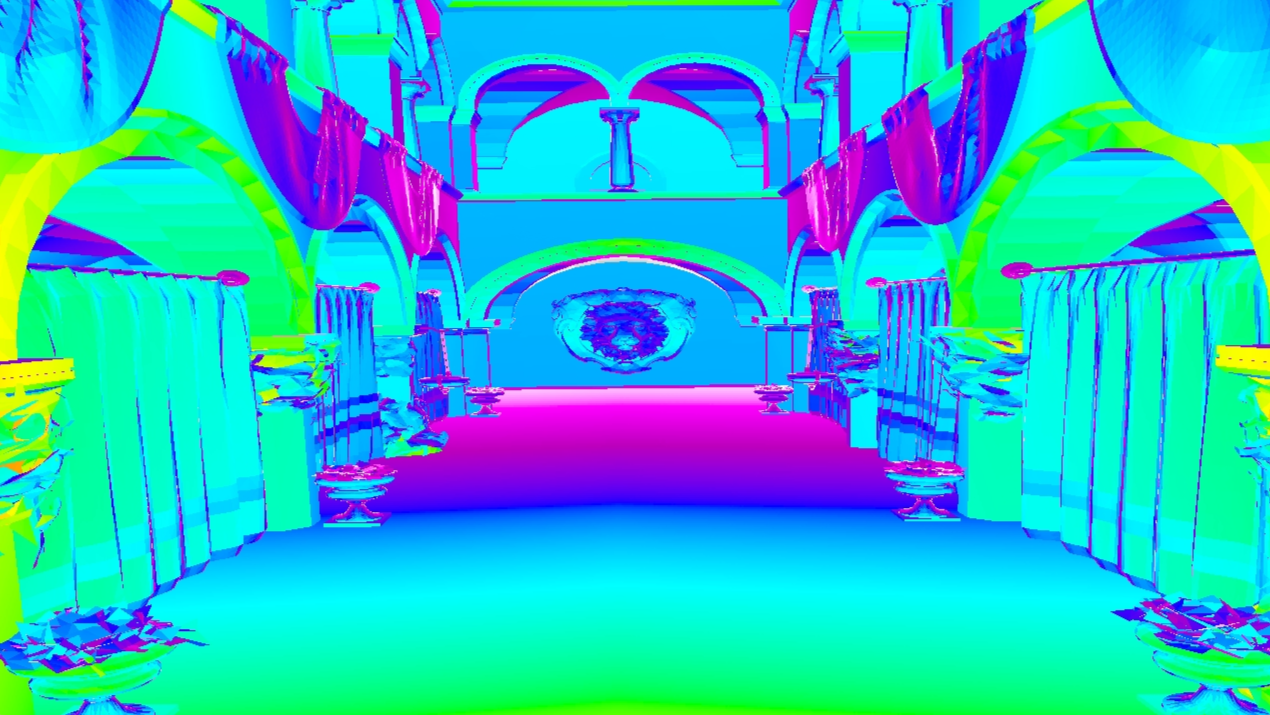
\includegraphics[width=0.45\textwidth]{1.4_mipmapLevels_LINEAR.png}
    }
    \subfigure[NEAREST]{
        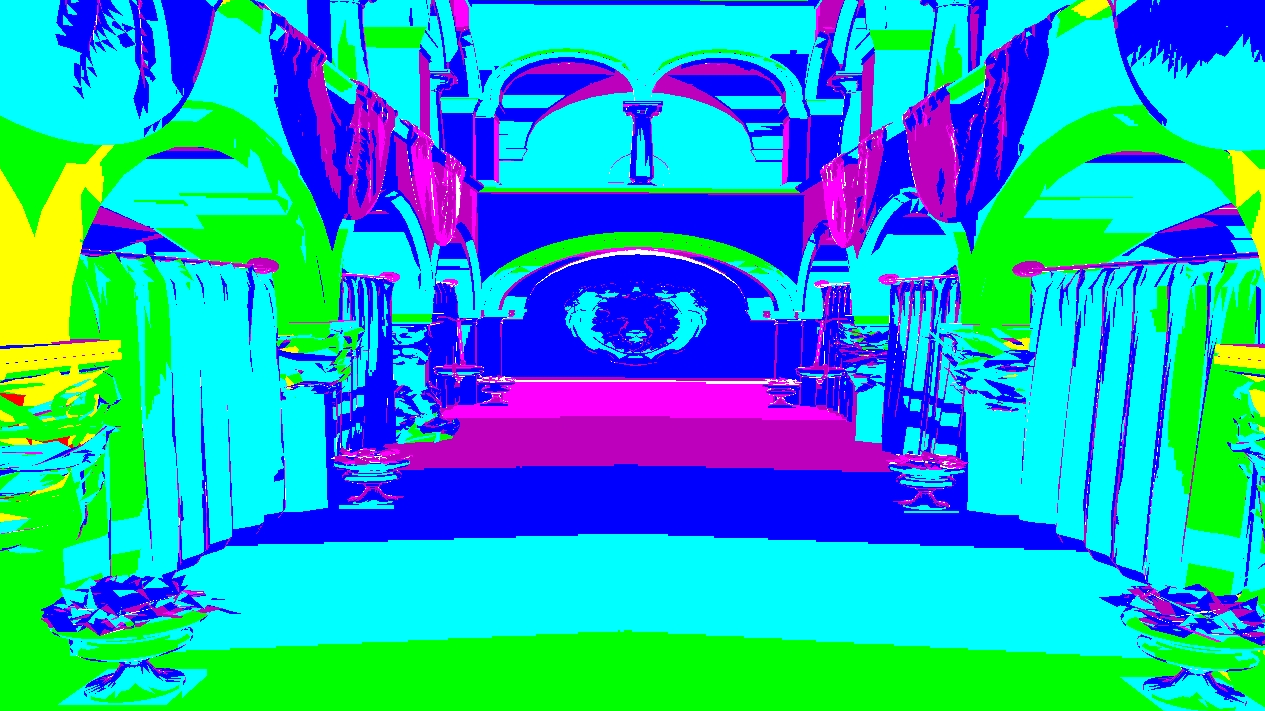
\includegraphics[width=0.45\textwidth]{1.4_mipmapLevels_NEAREST.png}
    }
    \caption{Two different mipmap mode}
\end{figure}

\subsection{Fragment depth}

\noindent In the `fragmentDepth.frag` shader, by calculating the result of `gl\_FragCoord.z / gl\_FragCoord.w`, the normalized device coordinate depth in clip space is obtained, and then divided by 100 to obtain a relatively suitable range, which is output as the color of the fragment.

\begin{lstlisting}
    // (X, Y, Z, W) -> (X/W, Y/W, Z/W, 1)
    float normalizedDepth = (gl_FragCoord.z / gl_FragCoord.w)/100.0;
    vec4 depthColor = vec4(normalizedDepth, normalizedDepth, normalizedDepth, 1.0);

    oColor = depthColor;
\end{lstlisting}

\noindent The resulting value is as shown in Figure 5.

\begin{figure}[htbp]
    \centering
    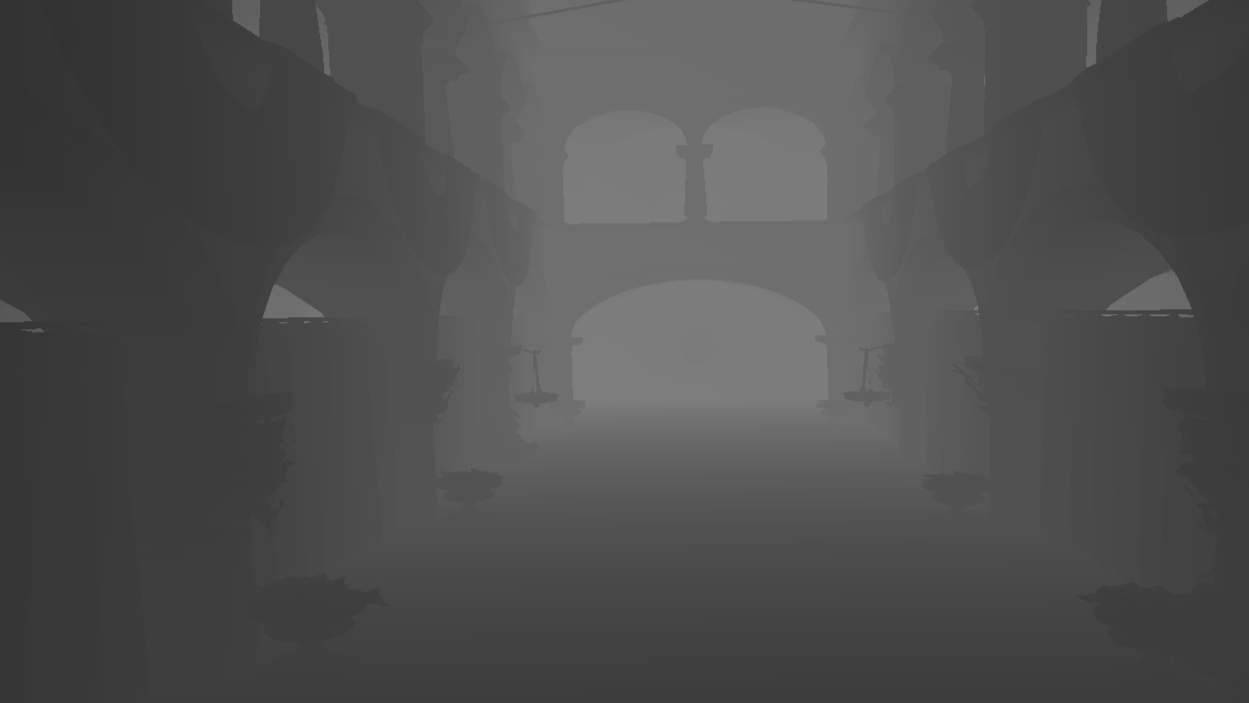
\includegraphics[width=9cm]{1.4_depthcolor.png}
    \caption{Fragment depth}
\end{figure}

\subsection{The partial derivatives of the per-fragment depth}

\noindent In the `partialDerivativesFragmentDepth.frag` shader, the depth value is calculated using `gl\_FragCoord.z / gl\_FragCoord.w`. Then, the partial derivatives are computed using the `dFdx()` and `dFdy()` methods. Finally, the derivatives are output as colors.

\begin{lstlisting}
    float depth = gl_FragCoord.z / gl_FragCoord.w;
    
    float depthDerivativeX = dFdx(depth);
    float depthDerivativeY = dFdy(depth);
    vec3 depthGradient = vec3(depthDerivativeX, depthDerivativeY, 0.0);
    
    vec3 color = abs(depthGradient);
    color = clamp(color, 0.0, 1.0);
    oColor = vec4(color, 1.0);
\end{lstlisting}

\noindent The resulting value is as shown in Figure 6.

\begin{figure}[htbp]
    \centering
    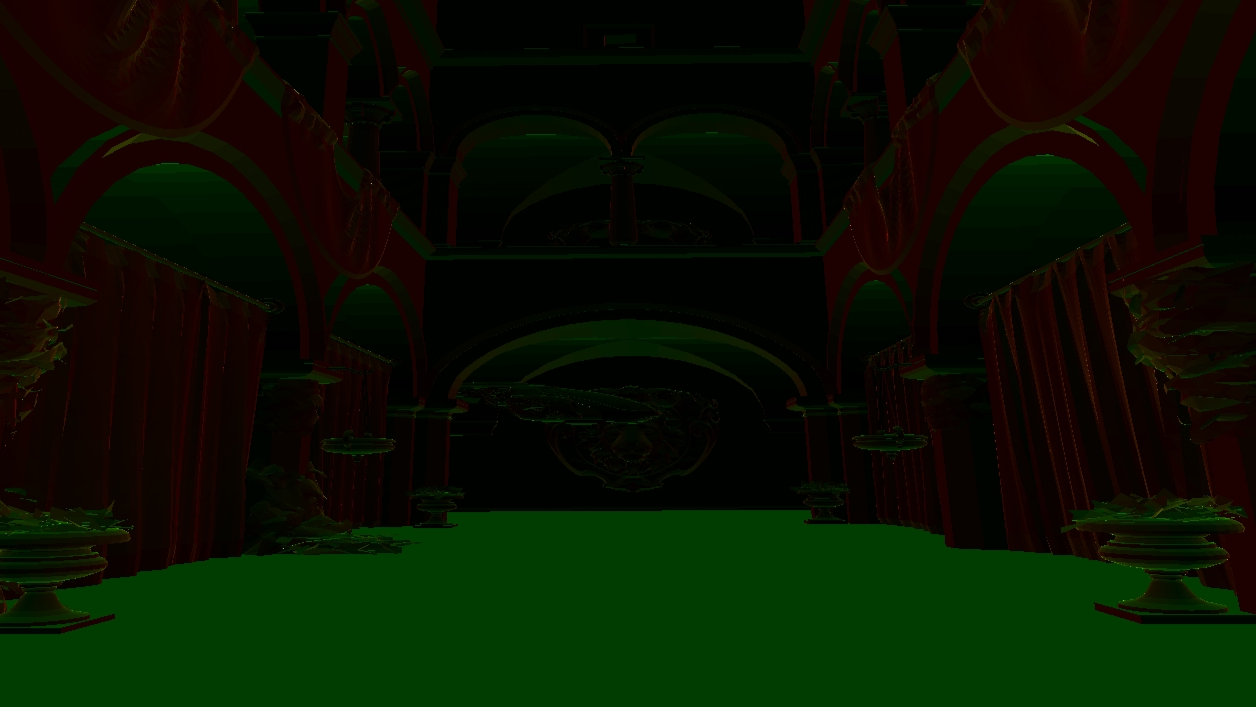
\includegraphics[width=9cm]{1.4_partialDerivativesFragmentDepth.png}
    \caption{The partial derivatives of the per-fragment depth}
\end{figure}

\section{Visualizing overdraw and overshading}

\noindent To visually clarify how drawn pixels are stacked together and the shading between different pixels, I enabled ColorBlend.

\begin{lstlisting}
#if CURRENT_VERSION == OVERDRAW_VISUALIZE || CURRENT_VERSION == OVERSHADING_VISUALIZE
    blendStates[0].blendEnable = VK_TRUE;
    blendStates[0].srcColorBlendFactor = VK_BLEND_FACTOR_ONE;
    blendStates[0].dstColorBlendFactor = VK_BLEND_FACTOR_DST_ALPHA;
    blendStates[0].colorBlendOp = VK_BLEND_OP_ADD;
    blendStates[0].srcAlphaBlendFactor = VK_BLEND_FACTOR_ONE;
    blendStates[0].dstAlphaBlendFactor = VK_BLEND_FACTOR_ZERO;
    blendStates[0].alphaBlendOp = VK_BLEND_OP_ADD; 
#else
    blendStates[0].blendEnable = VK_FALSE;
#endif
\end{lstlisting}

\noindent To prevent later-drawn pixels from covering previously drawn pixels in overdraw part, I disabled `depthTest` and `depthWrite` in the `create\_pipeline()` function.

\begin{lstlisting}
#if CURRENT_VERSION == OVERDRAW_VISUALIZE
    depthInfo.depthTestEnable = VK_FALSE;
    depthInfo.depthWriteEnable = VK_FALSE;
#else
    depthInfo.depthTestEnable = VK_TRUE;
    depthInfo.depthWriteEnable = VK_TRUE;
    depthInfo.depthCompareOp = VK_COMPARE_OP_LESS_OR_EQUAL;
    depthInfo.minDepthBounds = 0.f;
    depthInfo.maxDepthBounds = 1.f;
#endif 
\end{lstlisting}

\noindent In the `overDraw\_overShading.frag` shader, I set the color to dark green.

\begin{lstlisting}
	oColor = vec4(0,0.1,0,1.0);
\end{lstlisting}

\noindent The resulting value is as shown in Figure 7. 
I can observe that, compared to Overshading, the result of Overdraw shows deeper colors in areas with overlapping surfaces, whereas Overshading only displays colors on surfaces that are retained after passing the depth test.

\begin{figure}[htbp]
	\centering
	\subfigure[Baseline Overdraw]{
        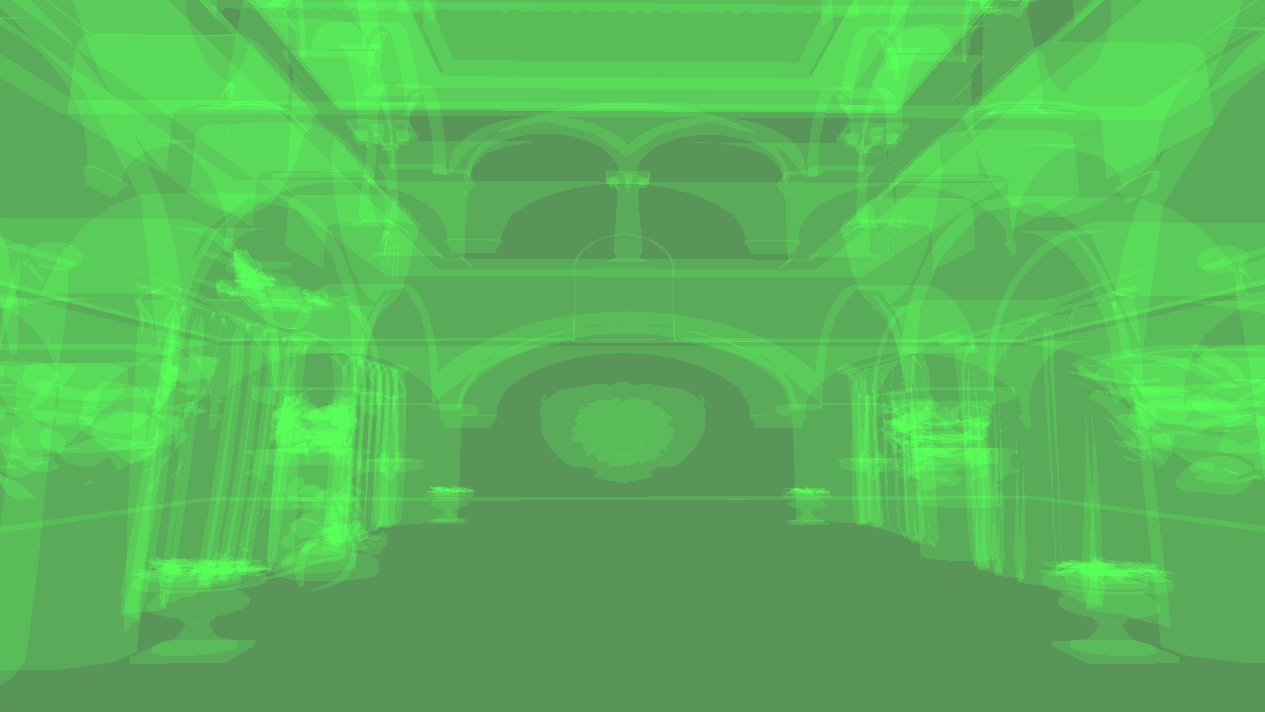
\includegraphics[width=0.45\textwidth]{1.5_overDraw.png}
    }
    \subfigure[Overshading]{
        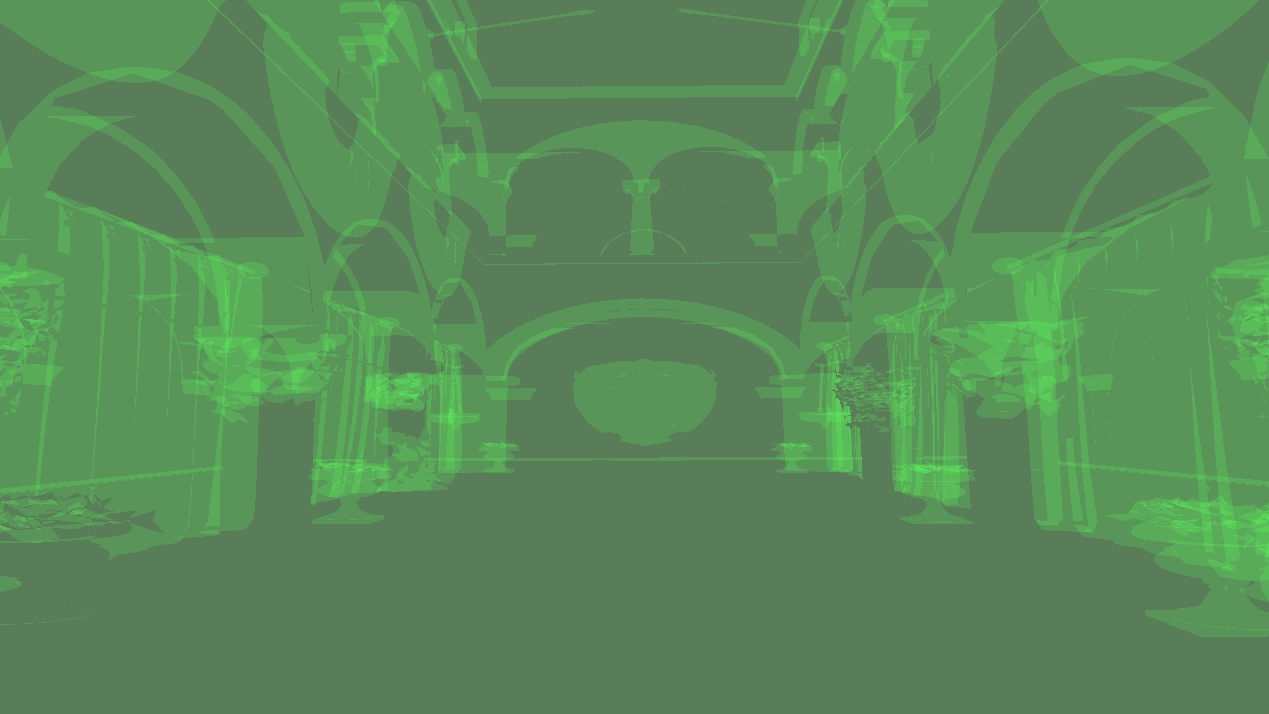
\includegraphics[width=0.45\textwidth]{1.5_overShading.png}
    }
    \caption{Baseline overdraw and Overshading}
\end{figure}

\section{Visualizing Mesh Density}

\noindent In the create\_pipeline() method in main.cpp, add the geometry shader to it.

\begin{lstlisting}
    lut::ShaderModule vert = lut::load_shader_module(aWindow, cfg::kVertShaderPath);
    lut::ShaderModule geom = lut::load_shader_module(aWindow, cfg::kMeshDensityShaderPath);
    lut::ShaderModule frag = lut::load_shader_module(aWindow, cfg::kFragShaderPath);
    
    VkPipelineShaderStageCreateInfo stages[3]{};
    stages[0].sType = VK_STRUCTURE_TYPE_PIPELINE_SHADER_STAGE_CREATE_INFO;
    stages[0].stage = VK_SHADER_STAGE_VERTEX_BIT;
    stages[0].module = vert.handle;
    stages[0].pName = "main";
    stages[1].sType = VK_STRUCTURE_TYPE_PIPELINE_SHADER_STAGE_CREATE_INFO;
    stages[1].stage = VK_SHADER_STAGE_GEOMETRY_BIT;
    stages[1].module = geom.handle;
    stages[1].pName = "main";
    stages[2].sType = VK_STRUCTURE_TYPE_PIPELINE_SHADER_STAGE_CREATE_INFO;
    stages[2].stage = VK_SHADER_STAGE_FRAGMENT_BIT;
    stages[2].module = frag.handle;
    stages[2].pName = "main";
\end{lstlisting}

\noindent And set pipeInfo.stageCount to 3 to specify the number of shader stages included in the pipeline.

\begin{lstlisting}
    VkGraphicsPipelineCreateInfo pipeInfo{};
    pipeInfo.sType = VK_STRUCTURE_TYPE_GRAPHICS_PIPELINE_CREATE_INFO;
    //pipeInfo.stageCount = 2;
    pipeInfo.stageCount = 3;
\end{lstlisting}

\noindent In the create\_scene\_descriptor\_layout() function, modify bindings[0].
stageFlags to inform Vulkan that the pipeline includes both the vertex shader and the geometry shader stages.

\begin{lstlisting}
//bindings[0].stageFlags = VK_SHADER_STAGE_VERTEX_BIT;
bindings[0].stageFlags = VK_SHADER_STAGE_VERTEX_BIT | VK_SHADER_STAGE_GEOMETRY_BIT;
\end{lstlisting}

\noindent Modify deviceFeatures.geometryShader in the create\_device() function in vulkan\_window.cpp to enable the device's geometry shader functionality.

\begin{lstlisting}
    deviceFeatures.geometryShader = VK_TRUE;
\end{lstlisting}

\noindent Create a new geometry shader to calculate the density of the mesh using the average length of its three edges and pass this value to the fragment shader.

\begin{lstlisting}    
  vec3 v0 = (gl_in[0].gl_Position).xyz;
  vec3 v1 = (gl_in[1].gl_Position).xyz;
  vec3 v2 = (gl_in[2].gl_Position).xyz;

  float a = length(v1 - v0);
  float b = length(v2 - v1);
  float c = length(v0 - v2);

  float avgEdgeLength = (a + b + c) / 3.0;
  
  for(int i = 0; i < 3; ++i) {
	density = avgEdgeLength;
    gl_Position = uScene.projCam * gl_in[i].gl_Position;
    EmitVertex();
  }
  EndPrimitive();
\end{lstlisting}

\noindent In the fragment shader, set colors for high-density and low-density grids, and output the color of the current fragment based on the current density for both high and low-density regions.

\begin{lstlisting}
    float normalized = 1.0 / (1.0 + exp(-1 * density));

    vec3 lowColor = vec3(0, 0, 0);
    vec3 highColor = vec3(0.8, 1.0, 0.8);
    vec3 finalColor = mix(lowColor, highColor, normalized);

    oColor = vec4(finalColor, 1.0);
\end{lstlisting}

\noindent The final output resembles Figure 8. By observing the grid density, I can discern a smiling face pattern on the cloth hanging from the wall.

\begin{figure}[htbp]
    \centering
    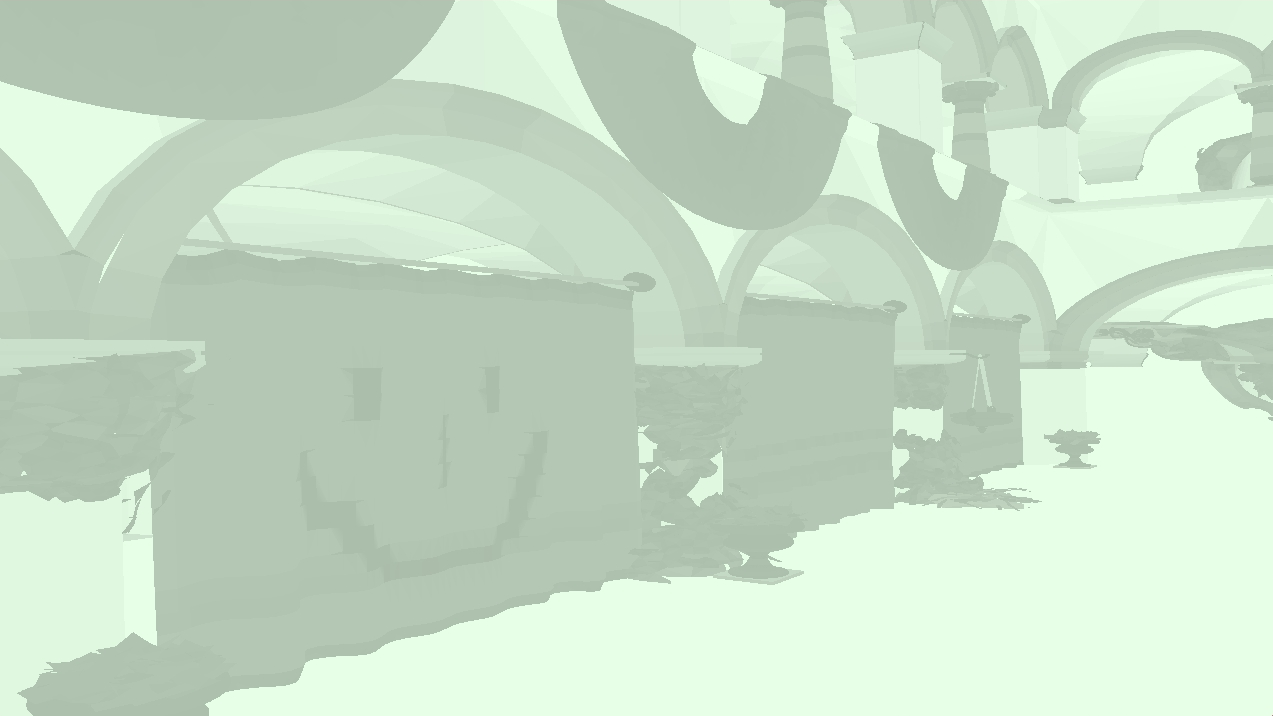
\includegraphics[width=9cm]{1.6_meshdensity_smile.png}
    \caption{Mesh density}
\end{figure}

\section{More overshading}

\noindent \dots\dots

\end{document}
